\documentclass[tikz, border=10pt]{standalone}
\usepackage{tikz}
\usetikzlibrary{arrows.meta}

\begin{document}
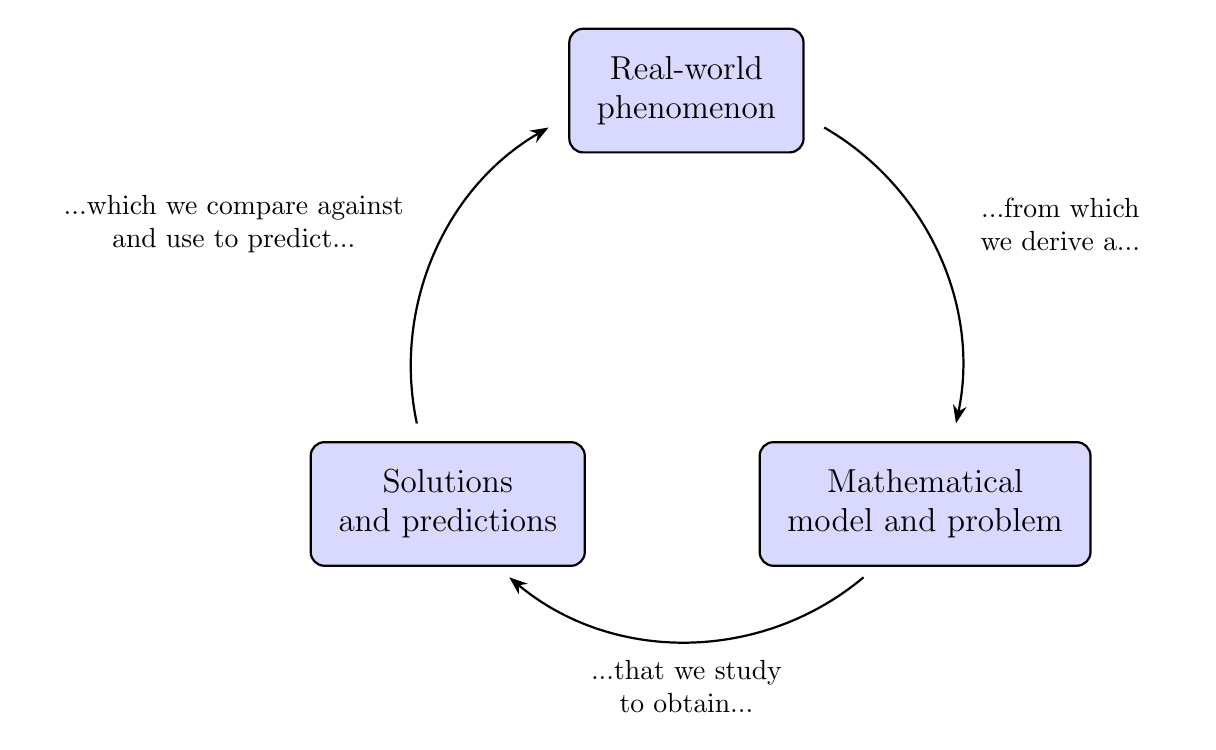
\begin{tikzpicture}[thick,
  box/.style={draw, fill=blue!15, rounded corners=5pt,
              minimum width=2.2cm, minimum height=1.1cm,
              align=center, font=\large, inner sep=10pt},
  arr/.style={-{Stealth}, thick}]

  \def\R{3.5}

  % --- Nodes at 12, 4, 8 o'clock ---
  \node[box] (A) at (90:\R)   {Real-world\\phenomenon};
  \node[box] (B) at (-30:\R)  {Mathematical\\model and problem};
  \node[box] (C) at (-150:\R) {Solutions\\and predictions};

  % --- Clockwise arcs using the arc command ---
  % Each arc runs clockwise (decreasing angle) between node centres,
  % shortened at both ends so the arrowhead clears the box border.
  \draw[arr]
    (60:\R)   arc[start angle=60,   end angle=-12,  radius=\R];
  \draw[arr]
    (-50:\R)  arc[start angle=-50,  end angle=-130, radius=\R];
  \draw[arr]
    (-168:\R) arc[start angle=-168, end angle=-240, radius=\R];

  % --- Labels at 2, 6, 10 o'clock, just outside the circle ---
  \node[draw=none, text width=3cm, anchor=west, align=center] at ( 30:{\R+0.1}) {...from which\\we derive a...};
  \node[draw=none, text width=3cm, anchor=north, align=center] at (270:{\R+0.1}) {...that we study\\to obtain...};
  \node[draw=none, text width=5cm, anchor=east, align=center] at (150:{\R+0.1}) {...which we compare against\\and use to predict...};

\end{tikzpicture}
\end{document}
